\documentclass[twoside,11pt]{homework}

\coursename{COMS 4771 Machine Learning 2020} 

\studname{Joseph High \& Eliza Mace}    % YOUR NAME GOES HERE
\studmail{jph2185,emm2314}% YOUR UNI GOES HERE
\hwNo{1}                   % THE HOMEWORK NUMBER GOES HERE
\date{\today} % DATE GOES HERE

% Uncomment the next line if you want to use \includegraphics.
\usepackage{graphicx}
%\usepackage{fancyhdr}
\usepackage{enumerate}
\usepackage{amsmath}

\begin{document}
\maketitle

\section*{Problem 1: Statistical Estimators}


\section*{Problem 1: Statistical Estimators}
\begin{enumerate}[(i)]
	\item
	\begin{equation*}
	P(X|\theta=(a,b))\propto
	\begin{cases}
	1 & a \leq x \leq b \\
	0 &\text{otherwise}
	\end{cases}
	\end{equation*}
	$\mathcal{L}(\theta)={\displaystyle \prod_{i=1}^{N} p(x_i|\theta)}={\displaystyle \prod_{i=1}^{N} \frac{1}{b-a}=\frac{1}{(b-a)^N}}$ \\[10pt]
	$a\leq min(x_1,...,x_N)$ and $b\geq max(x_1,...,x_N)$ \\[10pt]
	maximum likelihood ($\mathcal{L}$) is when $b-a$ is as small as possible, so $b=max(x_i)$ and $a=min(x_i)$\\[10pt]
	$MLE(\theta)=(min(x_i),max(x_i))$	
	\item Invariance property of MLE's \\
	if $g$ is one-to-one:\\
	$\mathcal{L}(\theta) = \mathcal{L}(g^(-1)(g(\theta)))$\\[10pt]
	Likelihood is maximized by $\theta_{ML}$:\\
	$\theta_{ML}=g^{-1}(ML(g(\theta)))$ \\[10pt]
	$g(\theta_{ML})=ML(g(\theta))$\\[10pt]
	if $g$ is many-to-one:\\
	HELP!
	\item For 1-dim Gaussian
	\begin{itemize}
		\item consistent and unbiased:
		$\mu = \frac{1}{N}{\displaystyle \sum_{i=1}^{N}x_i}$
		\item consistent, but not unbiased:
		$\mu = \frac{1}{N-1}{\displaystyle \sum_{i=1}^{N}x_i}$ and $\mu = \frac{1}{N}{\displaystyle \sum_{i=1}^{N}x_i+\frac{1}{N}}$
		\item not consistent, but unbiased:
		\item neither consistent, nor unbiased:
		$\mu = constant \neq \hat{\mu}$
	\end{itemize}
\end{enumerate}

\section*{Problem 2: On Forecasting Product Demand}
\begin{enumerate}
	\item 
	\begin{equation*}
	\begin{split}
	\pi(D) &= \int_{0}^{Q-1}[(P-C)\cdot D-C\cdot (Q-D)]\cdot f(D)dD+\int_{Q}^{\infty}(P-C)\cdot Q\cdot f(D)dD\\
	&= \int_{0}^{Q-1}[(P-C)D-C(Q-D)]\cdot f(D)dD+(P-C)\cdot Q[ 1-\int_{0}^{Q-1}f(D)dD]\\
	&=\int_{0}^{Q-1}P\cdot D\cdot f(D)dD-C\cdot Q\int_{0}^{Q-1}f(D)dD+(P-C)\cdot Q+(P-C)\cdot Q \int_{0}^{Q-1}f(D)dD\\
	&=(P-C)\cdot Q+P\int_{0}^{Q-1}D\cdot f(D) dD + [(P-C)\cdot Q-C\cdot Q]\int_{0}^{Q-1}f(D)dD\\
	&=(P-C)\cdot Q+P\int_{0}^{Q-1}D\cdot f(D)dD+[Q\cdot(P-2C)][F(Q-1)-F(0)]
	\end{split}
	\end{equation*}
	\item 
	\begin{equation*}
	\begin{split}
	\frac{d\pi}{dQ}&=(P-C)+P\cdot(Q-1)\cdot f(Q-1)+\frac{d}{dQ}[(P-2C)\cdot Q\cdot F(Q-1)-(P-2C)\cdot Q \cdot F(0)]\\
	\end{split}
	\end{equation*}
\end{enumerate}

\section*{Problem 3: Evaluating Classifiers}
\begin{enumerate}[(i)]
	\item We get an error when $x_i>t,y_i=y_2$ or when $x_i\leq t,y_i=y_1$\\
	\begin{equation*}
	\begin{split}
	P[f_t(X)\neq y]&=P[f_t(\vec{x})=y_1,Y=y_2|X=\vec{x}]+P[f_t(\vec{x})=y_2,Y=y_1|X=\vec{x}]\\
	&=P[x_i>t,Y=y_2|X=x_i]+P[x_i\leq t,Y=y_1|X=x_i]
	\end{split}
	\end{equation*}
	$f_t(x)$ is conditionally independent of $y$ given $x$
	\begin{equation*}
	\begin{split}
	P[f_t(x)\neq y]&=P[x_i>t|X=x_i]P[Y=y_2|X=x_i]+P[x_i\leq t|X=x_i]P[Y=y_1|X=x_i]\\
	&=\mathbb{1}(x_i>t)P[Y=y_2,X=x_i]+(1-\mathbb{1}(x_i>t))P[Y=y_i|X=x_i]
	\end{split}
	\end{equation*}
	\item optimal threshold
	\item bayes error rate
\end{enumerate}

\section*{Problem 4: Analyzing iterative optimization}
\begin{enumerate}[(i)]
	\item symmetric positive semidefnite
	\item induction
	\item eigenvalues
	\item proof
\end{enumerate}

\section*{Problem 5: Designing socially aware classifiers}

\begin{enumerate}[(i)]
	\item It is not enough just to remove the sensitive attribute \emph{A} from the dataset because it is possible that other attributes in the feature vector are correlated with this attribute.
	\item Demographic parity
	\item equivalence relationship
	\item classifiers
	\item 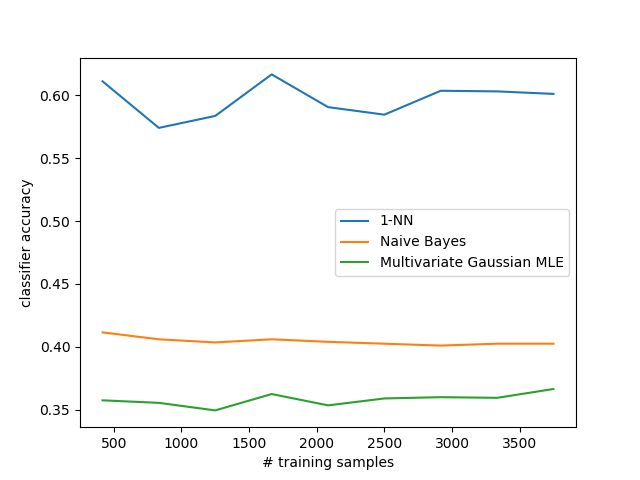
\includegraphics[width=\textwidth]{compas.png}
	\item positive rate across sensitive attribute
	\item real-world
\end{enumerate}

\section*{Problem 6: Email spam classification case study}

\begin{enumerate}[(i)]
	\item Bag-of-words
	\item classifiers
	\item Naive bayes is best!
\end{enumerate}

\end{document} 
